\chapter{Dynamic Grid}\label{ch:dynamicGrid}

\textit{Often in math, you should view the definition not as a starting point, but as a target. Contrary to the structure of textbooks, mathematicians do not start by making definitions and then listing a lot of theorems, and proving them, and showing some examples. The process of discovering math typically goes the other way around. They start by chewing on specific problems, and then generalising those problems, then coming up with constructs that might be helpful in those general cases,and only then you write down a new definition (or extend an old one). - Grant Sanderson (AKA 3Blue1Brown) https://youtu.be/O85OWBJ2ayo?t=359}

This chapter provides an extended summary to the paper ``Dynamic grids for Finite-Difference Schemes in Musical Instrument Simulations'' \citeP[G]. The paper presents a novel method to smoothly add and remove grid points from a FD scheme which allows for dynamic parameter variations without compromising stability or quality of the simulation (see Section \ref{sec:quality1DWave}). 

After a brief introduction  and summary of the method, the chapter will extend on paper \citeP[G] by providing some design considerations as a result of iterations done as well as providing details on the implementation of the displacement correction and the modal analysis shown in the paper. 

\section{Background and motivation}
Simulating musical instruments using physical modelling -- as mentioned in Chapter \ref{ch:physMod} -- allows for manipulations of the instrument that are impossible in the physical world. Examples of this are changes in material density or stiffness, cross-sectional area (1D), thickness (2D) and size of the system in general. 



\subsection{Examples}
Apart from being potentially sonically interesting, there are examples in the physical world where certain aspects of the instrument are manipulated in real-time.

Tension in a string is changed when tuning it

Some artists even use this in their performances \cite{Gomm2011, Mayer2008}
Or gr4yhound: https://www.youtube.com/watch?v=fSQ9Dg65EFo

The hammered dulcimer is another example where the strings are tensioned over a bridge where one can play the string at one side of the bridge, while pushing down on the same string on the other side \cite{Glenn2014}.

\noindent 1D:
\begin{itemize}
    \item Trombone
    \item Slide whistle
    \item Guitar strings
    \begin{itemize}
        \item Fretting finger pitch bend
        \item Above the nut \cite{Mayer2008}
        \item Tuning pegs directly \cite{Gomm2011}
    \end{itemize}
    \item Hammered dulcimer \cite{Glenn2014}
    \item Erhu? 
\end{itemize}
%
2D: 
\begin{itemize}
    \item Timpani
    \item Bodhr\'an: https://youtu.be/b9HyB5yNS1A?t=146
    \item Talking drum (hourglass drum): https://youtu.be/B4oQJZ2TEVI?t=9
    \item Flex-a-tone (could also be 1D tbh..): https://www.youtube.com/watch?v=HEW1aG8XJQk.
\end{itemize}

A more relevant example is that of the trombone, where the size of the instrument is changed in order to play different pitches. Modelling this using FDTD methods would require

% \section{Issues with FDTD methods}


In his thesis, Harrison points out that in order to model the trombone, grid points need to be introduced 


Something about time-dependent variable coefficient Stokes flow:
https://arxiv.org/abs/1010.2832

Time-varying propagation speed in waveguides: https://quod.lib.umich.edu/cgi/p/pod/dod-idx/fractional-delay-application-time-varying-propagation-speed.pdf?c=icmc;idno=bbp2372.1997.069;format=pdf

Special boundary conditions (look at!):
Modeling of Complex Geometries and Boundary Conditions in Finite Difference/Finite Volume Time Domain Room Acoustics Simulation (\url{https://www.researchgate.net/publication/260701231_Modeling_of_Complex_Geometries_and_Boundary_Conditions_in_Finite_DifferenceFinite_Volume_Time_Domain_Room_Acoustics_Simulation})



\section{Summary}
The variations are assumed to be at sub-audio rate (i.e., human gestural control) so that analysis techniques are still valid to some degree.


Consider the 1D wave equation  as presented in Section \ref{sec:1DWave}, describing the motion of a system of length $L$, its state described by $q = q(x,t)$ defined for $t\geq 0$ and $x\in\D$ with domain $\D = [0, L]$. This state variable can be discretised to a grid function $\qln$ with $n\in \mathbb{N}^0$ and $l \in \{0, \hdots, N\}$ with $N$ being tthe number of intervals between the grid points. The PDE in \eqref{eq:1DwavePDE} can then be discretised to the following FD scheme
\begin{equation}
    \dtt \qln = c^2\dxx \qln.
\end{equation}

Rather than working with this scheme directly, paper \citeP[G] proposes to split it into two to get the following system 
\begin{subequations}
    \begin{equation}
        \dtt \ulun = c^2\dxx \ulun,
        \dtt \wlwn = c^2\dxx \wlwn.
    \end{equation}
\end{subequations}

\section{Iterations}
Iterations have been:
\begin{itemize}
    \item Interpolated boundary conditions
    \item Linear interpolation
\end{itemize}

\todo{These sections are taken from the JASA appendix} In this appendix, some iterations done over the course of this project will be shown in more detail. In the following, the 1D wave equation with a wave speed of $c = 1470$ m/s, a length of $L = 1$ m, Dirichlet boundary conditions and a sample rate of $f_\text{s} = 44100$ Hz is considered, and -- through Eq. \eqref{eq:compactLambda} -- satisfies the CFL condition with equality. These values result in $N = 30$, or a grid of 31 points including the boundaries. Then, the wave speed is decreased to $c \approx 1422.6$ m/s, i.e., the wave speed that results in $N=31$ and satisfies the stability condition with equality again. 

\subsection{Full-grid interpolation}
One way to go from one grid to another is performing a full-grid interpolation \cite[Chap. 5]{theBible}. If the number of points changes according to Eq. \eqref{eq:orderOfCalcGrid}, i.e., if $N^n \neq N^{n-1}$ the full state of the system ($u_l^n, u_l^{n-1}\ \forall l$)  can be interpolated to the new state. See Figure \ref{fig:fullGrid}. 

\begin{figure}[ht]
    \centering

%% \reprintcolumnwidth is the same in preprint and reprint for
%% ease of use for authors:
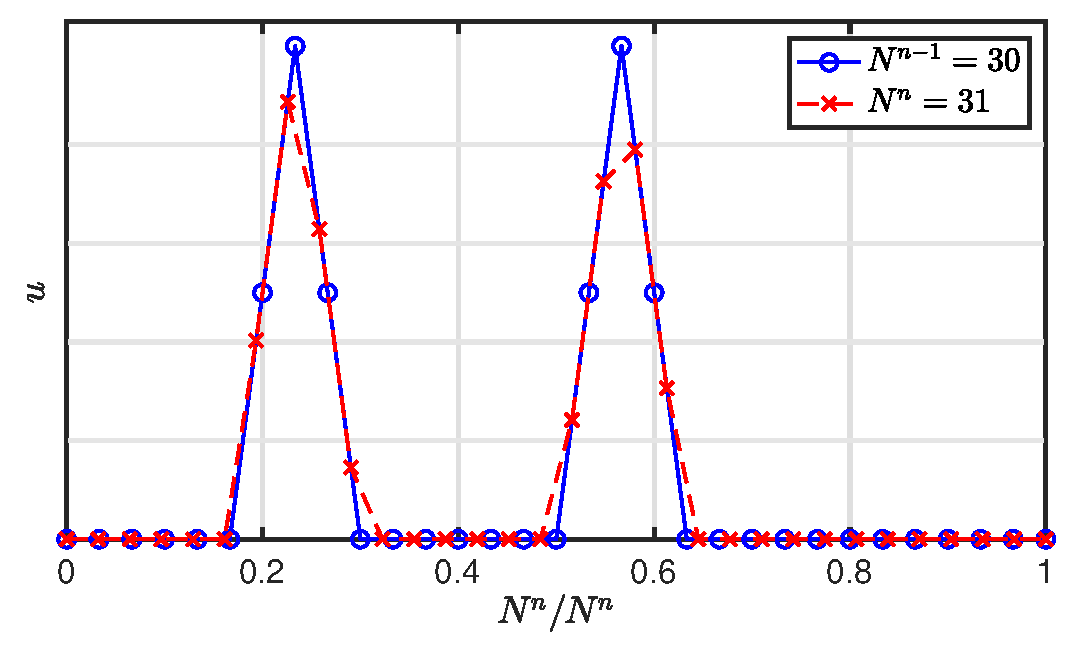
\includegraphics[width=0.5\textwidth]{figures/contributions/dynamicgrid/fullGrid.eps}
\caption{\label{fig:fullGrid}{Upsampling $u$ (with an arbitrary state) using (linear) full-grid interpolation with $N^{n-1} = 30$ and $N^n = 31$. The horizontal axis is normalised with respect to $N^n$.}}
\end{figure} 

An issue that arises using this method is that the Courant number $\lambda$ will slightly deviate from the CFL condition as $c$ changes. Using Eq. \eqref{eq:compactLambda} with $L/ck$ approaching $31$ (from below), the minimum value of $\lambda \approx 30/31 \approx 0.9677$.
%\footnote{Eq. \eqref{eq:orderOfCalcGrid} can be compactly rewritten as $\lambda = \frac{ck}{L}\cdot \text{floor}\left(\frac{L}{ck}\right)$. As $L/ck$ approaches $31$ (from below), $\lambda \approx \frac{30}{31}$.}
This, employing Eq. \eqref{eq:fmax}, has a maximum frequency output of $f_\text{max} \approx 18,475$ Hz. 
%For slightly lower values of $c$, $N = 31$ and $\lambda \approx 1$. 
The Courant number will deviate more for higher values of $c$ and thus lower values for $N$ -- for instance, if $N$ approaches $11$ (from below), $\lambda \approx 10/11 \approx 0.9091$ and $f_\text{max} \approx 16,018$ Hz.

Another problem with full-grid interpolation, is that it has a low-passing effect on the system state, and thus on the output sound. %Figure \ref{fig:fullGrid} shows the biggest changes are in the state are at the locations with the biggest difference between the states of consecutive grid points.
Furthermore, this state-interpolation causes artefacts or `clicks' in the output sound as the method causes sudden variations in the states.  

All the aforementioned issues could be solved by using a (much) higher sample rate and thus more grid points, but this would render this method impossible to work in real time.

\subsection{Adding and removing points at the boundary}\label{sec:addAtBoundary}
To solve the issues exhibited by a full-grid interpolation, points can be added and removed at a single location and leave most points unaffected by the parameter changes. A good candidate for a location to do this is at a fixed (Dirichlet) boundary. The state $u$ at this location is always $0$ so points can be added smoothly. 

As $c$ decreases, $h$ can be calculated according to Eq. \eqref{eq:orderOfCalcGrid} and decreases as well.

This has a physical analogy with tuning a guitar string. Material enters and exits the neck (playable part of the string) at the nut, which in discrete time means grid points appearing and disappearing at one boundary.

To yield smooth changes between grid configurations, an interpolated boundary has been developed, the possibility of which has been briefly mentioned in \cite[p. 145]{theBible}. The Dirichlet condition in Eq. \eqref{eq:contDirichlet} can be extended to be the simply supported boundary condition:
\begin{equation}
    u(x, t) = \frac{\partial^2}{\partial x^2}u(x, t) = 0 \quad \text{where} \quad x = 0, L,
\end{equation}
or, when discretised,
\begin{equation}\label{eq:simplySupportedDiscrete}
    u_l^n = \delta_{xx}u_l^n = 0, \quad \text{where} \quad l = 0, N.
\end{equation}
This means that on top of that the state of the boundary should be $0$, the curvature around it should also be $0$. One can again solve for the virtual grid points at the boundary locations, yielding
\begin{equation}
    u_{-1}^n = -u_1^n \quad \text{and} \quad u_{N+1}^n = -u_{N-1}^n.
\end{equation}
This is visualised in Figure \ref{fig:simplySupportedBound}.

\begin{figure}
    \centering
    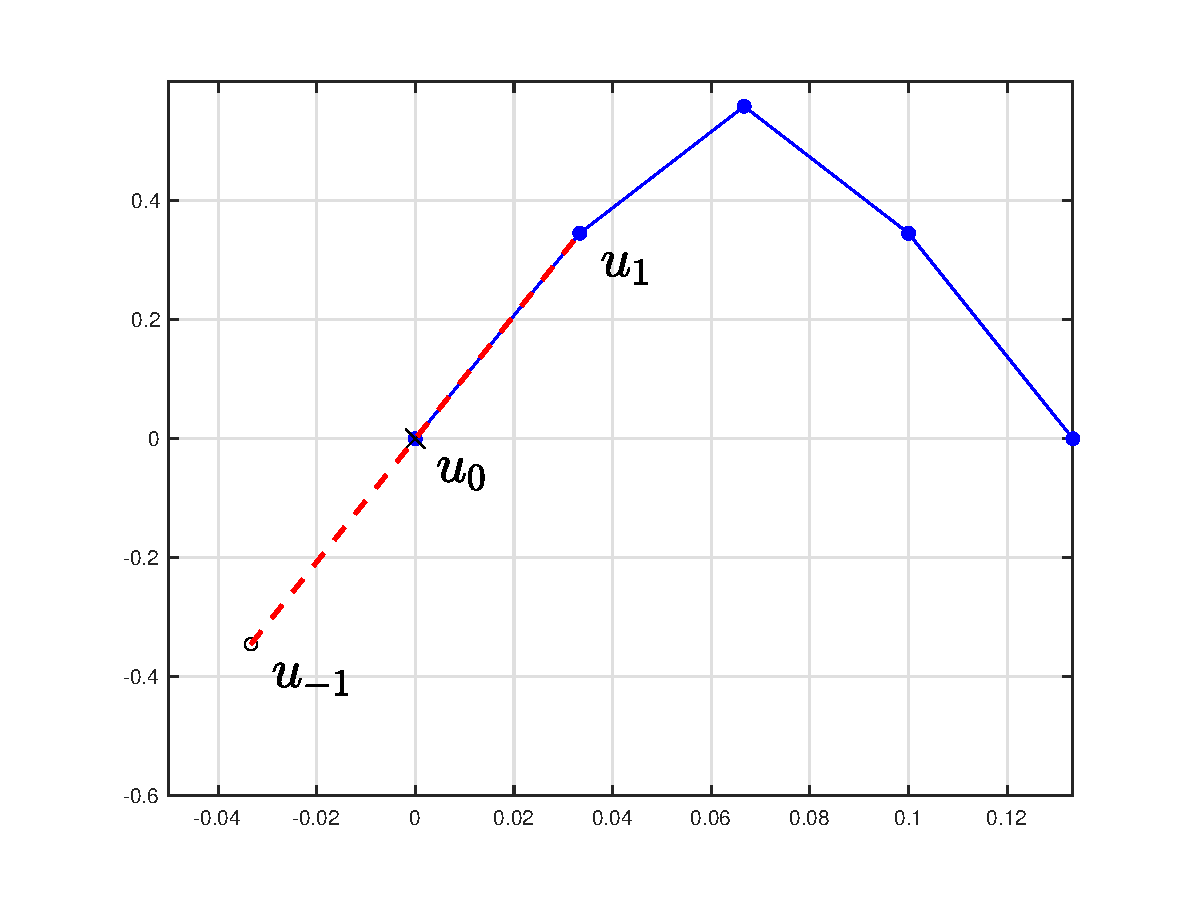
\includegraphics[width=0.7\textwidth]{figures/contributions/dynamicgrid/simplySupportedBoundary.eps}
    \caption{\label{fig:simplySupportedBound}{The simply supported boundary condition: both the state and the curvature at the boundary -- at $l=0$ -- should be $0$.}}
\end{figure} 

If the flooring operation in Eq. \eqref{eq:numberOfIntervals} is removed this introduces a fractional number of grid points.


The by-product of using a fractional $N$ this is that the CFL condition in \eqref{eq:CFL} can now always be satisfied with equality no matter what the wave speed is.

An issue with this method is that removing points is much harder than adding.

their interactions change through a change in the grid spacing and wave speed. This interaction, though, is defined by $\lambda$ which 

\begin{figure}
    \centering
%% \reprintcolumnwidth is the same in preprint and reprint for
%% ease of use for authors:
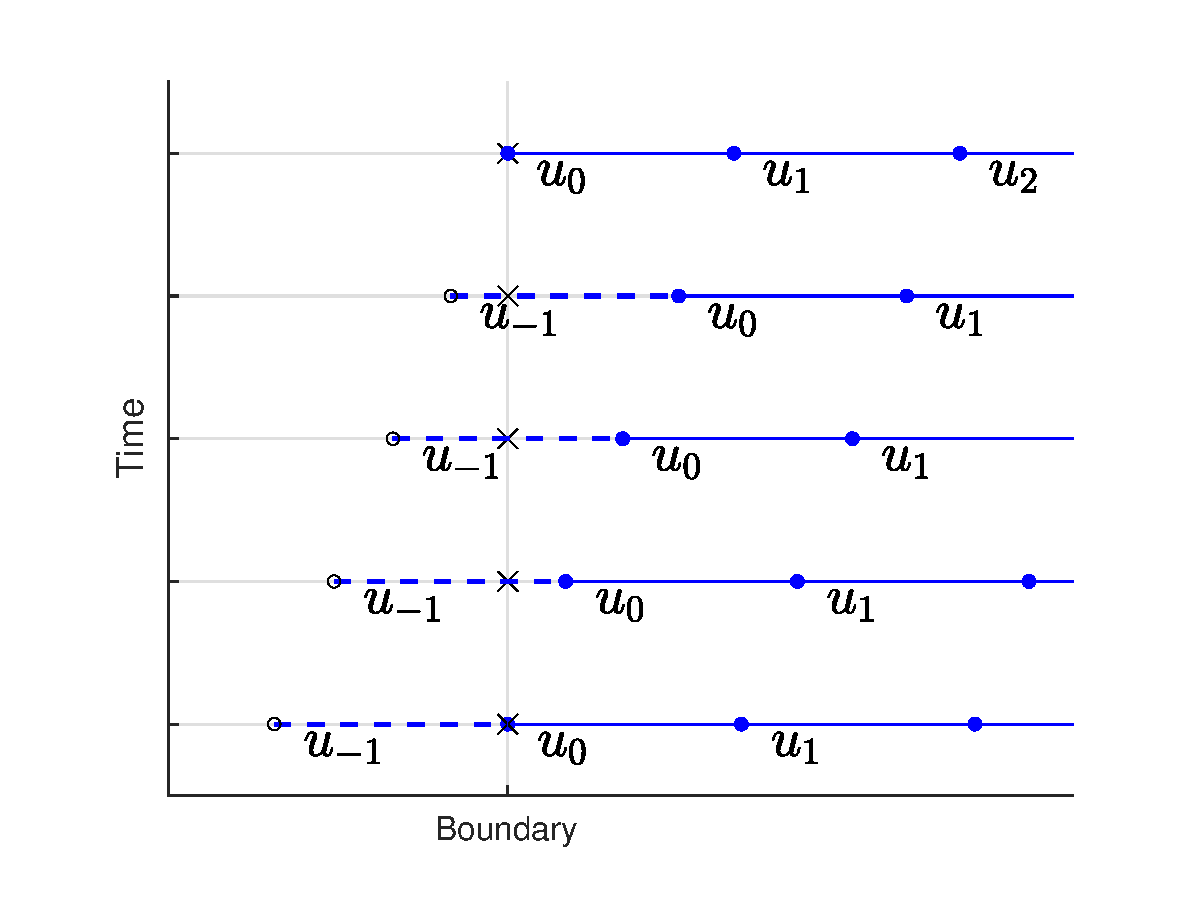
\includegraphics[width=0.7\textwidth]{figures/contributions/dynamicgrid/boundaryGrid.eps}
\caption{\label{fig:changingBoundary}{The grid changing over time}}
\end{figure}

\subsection{Cubic interpolation}

\subsection{Sinc interpolation}


\section{Displacement correction implementation} 
One detail that was not provided in paper \citeP[G], is the impelmentation of the displacement correction.
When the wave speed is increased and points are removed, it is not necessarily true that $u_M = w_0$ at the time of removal and the rigid connection in \eqref{eq:rigid} is violated. On top of the virtual grid point ``generation'' from the interpolation described above, one could add a connection force that is dependent on how close the inner boundaries $u_M$ and $w_0$ are.

We can extend \eqref{eq:systemHalfStrings} to have a spring force between $u_M$ and $w_0$ as
\begin{equation}\label{eq:dispCorrSyst}
    \begin{cases}
        \delta_{tt}u^n &= c^2\delta_{xx}u^n + J(x_{u_M})F\\
        \delta_{tt}w^n &= c^2\delta_{xx}w_0^n - J(x_{w_0})F
    \end{cases}
\end{equation}
with 
\begin{equation}\label{eq:corrForceNoDamp}
    F = \beta \mu_{t\cdot}\eta^n.
\end{equation}
Here,
\begin{equation}\label{eq:etaCorrDef}
    \eta^n \triangleq w_0^n - u_M^n
\end{equation}
is the difference in displacement between the inner boundaries
and $\beta = \beta(\alpha)$ 
acts as a spring coefficient that is a function of the distance between the inner boundaries along the grid, i.e., $\alpha$. Furthermore, the centred temporal averaging operator $\mu_{t\cdot}$ is used in \eqref{eq:corrForceNoDamp} to ensure stability \cite{Bilbao2009Modular}.

We then continue by finding a definition for $\beta$ that is inversely proportional to $\alpha$, i.e., the smaller $\alpha$ is the higher the `correction' effect, ideally approaching an infinite stiffness, or rigid connection, when $\alpha = 0$ and no stiffness when $\alpha \rightarrow 1$. This can be achieved by defining $\beta = \beta(\alpha)$ as
\def\plusEps{+ \epsilon}
% \def\plusEps{};
\def\alfPlusEps{(\alpha \plusEps)}
% \def\alfPlusEps{\alpha}
\begin{equation}\label{eq:betaDef}
    \beta = \frac{1 - \alpha}{\alpha \plusEps},
\end{equation}
with $0<\epsilon \ll 1$ to prevent a division by 0. It will be shown that when calculating the force after expansion, a division by 0 can be prevented and $\epsilon = 0$ will still yield a defined solution. We can observe that when $\alpha = 0$ and the correction effect needs to be at a maximum, $\beta\rightarrow \infty$. When $\alpha \rightarrow 1$, $\beta \rightarrow 0$.

We can also add a damping term to \eqref{eq:corrForceNoDamp} which is also scaled by $\beta$ as
\begin{equation}\label{eq:corrForce}
    F = \beta \left(\mu_{t\cdot}\eta^n +\sigma_0\delta_{t\cdot}\eta^n \right),
\end{equation}
where $\sigma_0$ is the damping coefficient. Then, we can solve for $\eta^{n+1}$ 
\begin{align}
    F &= \beta\left(\frac{1}{2}\left(\eta^{n+1}+\eta^{n-1}\right) + \frac{\sigma_0}{2k}\left(\eta^{n+1}-\eta^{n-1}\right)\right)\nonumber\\
    F&= \left(\frac{\beta (1 + \sigma_0/k)}{2}\right)\eta^{n+1} + \left(\frac{\beta (1 - \sigma_0/k)}{2}\right) \eta^{n-1}\nonumber\\
    \xLeftrightarrow{\mystrut\ \text{Eq. \eqref{eq:betaDef}}\ } \quad \eta^{n+1} &= \left(\frac{2
    \alfPlusEps}{(1+\sigma_0/k)(1-\alpha)}\right)F - \underbrace{\frac{1-\sigma_0/k}{1+\sigma_0/k}}_{r}\eta^{n-1}.\label{eq:etaSolut1}
\end{align}
Using superscript $\text{I}$ to denote an intermediate state describing of $u^{n+1}_M$ and $w^{n+1}_0$ without the connection force (see \eqref{eq:resultOneConnectedPoint}), we also know, through Eq. \eqref{eq:etaCorrDef}, that 

\begin{align}
    \eta^{n+1} &= w_0^\text{I}-\frac{k^2}{h}F-\left(u_M^\text{I}+\frac{k^2}{h}F\right)\nonumber\\
    \eta^{n+1} &= w_0^\text{I} - u_M^\text{I} - \frac{2k^2}{h}F,\label{eq:etaNext}
\end{align}
which can be set equal to \eqref{eq:etaSolut1} and solved for $F$ according to 

\begin{align*}
    \left(\frac{2
    \alfPlusEps}{(1+\sigma_0/k)(1-\alpha)}\right)F - r \eta^{n-1} &= w_0^{I} - u_M^{I}- \frac{2k^2}{h}F\\
    \left(\frac{2h
    \alfPlusEps + 2k^2(1+\sigma_0/k)(1-\alpha)}{h(1+\sigma_0/k)(1-\alpha)}\right)F &= w_0^{I} - u_M^{I}+r\eta^{n-1}\\
    F &= \left(w_0^{I} - u_M^{I}+r\eta^{n-1}\right)\left(\frac{h(1+\sigma_0/k)(1-\alpha)}{2h \alfPlusEps + 2k^2(1+\sigma_0/k)(1-\alpha)}\right).
\end{align*}
It is clear now that no matter the value of $\alpha$, no division by 0 will occur, so $\epsilon = 0$ is still defined. The final equation for $F$ can thus be written as
\begin{equation}\label{eq:finalForce}
    F = \left(w_0^{I} - u_M^{I}+r\eta^{n-1}\right)\underbrace{\left(\frac{h(1+\sigma_0/k)(1-\alpha)}{2h\alpha + 2k^2(1+\sigma_0/k)(1-\alpha)}\right)}_{\Psi}.
\end{equation}
This can then be filled into \eqref{eq:dispCorrSyst} and used to get $u_M^{n+1}$ and $w_0^{n+1}$ respectively. \SWcomment[Using $\alpha = 0$ and $\sigma_0 = 0$ as a test case to see what would happen to the scheme at the inner boundaries when they perfectly overlap (and without damping, just restoring force), we get that $r = 1$ and \eqref{eq:finalForce} becomes
\begin{align*}
    F &= \left(w_0^{I} - u_M^{I}+\eta^{n-1}\right)\left(\frac{h}{2k^2}\right)\\
    \xLeftrightarrow{\mystrut\ \text{Eq. \eqref{eq:etaNext}}\ } \quad F &= \left(\eta^{n+1} + \frac{2k^2}{h}F + \eta^{n-1}\right)\left(\frac{h}{2k^2}\right)\\
    F - F &= \eta^{n+1} + \eta^{n-1}\\
    2\mu_{t\cdot}\eta^n &= 0\\
    \mu_{t\cdot}\eta^n &= 0
\end{align*}
showing that when $\alpha = 0$, the $\eta^n$ should be 0 and thus boils down to a rigid connection.]

\subsubsection{Modal analysis}
Due to the damping that is present in the system, it needs to be written in one-step form. Recalling \eqref{eq:uVecDef} we can write \eqref{eq:dispCorrSyst} in vector-matrix form
\begin{equation}\label{eq:formForOneStep}
    \A \U^{n+1} = \B \U^n + \C\U^{n-1}
\end{equation}
and rewrite to one-step form as \SWcomment[decapitalise u!]
\begin{equation}\label{eq:oneStepForm}
    \underbrace{\begin{bmatrix}
        \U^{n+1}\\
        \U^n
    \end{bmatrix}}_{\mathbf{W}^{n+1}} = 
    \underbrace{\begin{bmatrix}
        \A^{-1}\B & \A^{-1}\C\\
        \I & \mathbf{0}
    \end{bmatrix}}_{\Q}
    \underbrace{\begin{bmatrix}
        \U^n\\
        \U^{n-1}
    \end{bmatrix}}_{\mathbf{W}^n}
\end{equation}

The most straightforward way to obtain the matrices, is to expand the forces in system \eqref{eq:dispCorrSyst} directly. 
% \begin{equation}
%     \begin{cases}
%         \delta_{tt}u^n &= c^2\delta_{xx}u^n + J(x_{u_M})\frac{\beta}{2}(\eta^{n+1} + \eta^{n-1} + \sigma_0/k (\eta^{n+1} - \eta^{n-1}))\\
%         \delta_{tt}w^n &= c^2\delta_{xx}w_0^n - J(x_{w_0})\frac{\beta}{2}(\eta^{n+1} + \eta^{n-1} + \sigma_0/k (\eta^{n+1} - \eta^{n-1}))
%     \end{cases}
% \end{equation}
% and
Recalling $\U$ from \eqref{eq:uVecDef} (of size $\mathcal{M} = M+M_w$) and including the virtual grid point definitions encapsulated in $\B_2$, we can rewrite the system to
\begin{equation}
    \I\U^{n+1} = \B_2\U^n - \I\U^{n-1} + (\J\boldsymbol{\eta})\frac{\beta k^2}{2}\left((1+\sigma_0/k)\U^{n+1} + (1-\sigma_0/k)\U^{n-1}\right)
\end{equation}
where 
\begin{equation}
    \J = [\mathbf{0}_{M-1}, 1/h, -1/h, \mathbf{0}_{M_w-1}]^T
\end{equation}
where $\mathbf{0}_i$ is a row-vector of zeros with length $i$ and
\begin{equation}
    \boldsymbol{\eta} = [\mathbf{0}_{M-1}, -1, 1, \mathbf{0}_{M_w-1}].
\end{equation}
vectorising the effect of \eqref{eq:etaCorrDef} on $\U$. Note that as $\J$ is a column vector and $\boldsymbol{\eta}$ a row vector, the multiplication of the two yields an $\mathcal{M}\times\mathcal{M}$ matrix.

Then refactoring to the form in \eqref{eq:formForOneStep} and using identity matrix $\I$ with size $\mathcal{M} \times \mathcal{M}$ yields the following matrices
% \begin{equation}
%     \underbrace{\left(\I - \frac{\beta k^2 (1+\sigma_0/k)}{2}\J\boldsymbol{\eta}\right)}_{\A}\U^{n+1} = \underbrace{\mathbf{B}_2}_{\B}\U^n +\underbrace{\left(- \I - \frac{\beta k^2 (1-\sigma_0/k)}{2}\J\boldsymbol{\eta}\right)}_{\C} \U^{n-1}
% \end{equation}

\begin{equation}
    \A = \I - \frac{\beta k^2 (1+\sigma_0/k)}{2}\J\boldsymbol{\eta}, \qquad \B = \mathbf{B}_2, \qquad \text{and} \qquad \C = -\left(\I - \frac{\beta k^2 (1-\sigma_0/k)}{2}\J\boldsymbol{\eta}\right)
\end{equation}
Although substituting these definitions into \eqref{eq:oneStepForm} gives an identical result to the matrix definitions above (comparisons show a difference between the $\Q$ matrices around machine precision), $\beta$ can still go to infinity. In this case, $\epsilon \neq 0$ in \eqref{eq:betaDef}. 

\section{%Modal 
Analysis and experiments}
\subsection{Interpolation technique}
\subsection{Interpolation range}
\subsection{Location}
... where to add and remove points

Using the whole range, we can still add/remove points at the sides. 

\section{Discussion and conclusion}\label{sec:conclusion}